%; whizzy chapter -dvi
% -initex iniptex -latex platex -format platex -bibtex jbibtex -fmt fmt
% 以上 whizzytex を使用する場合の設定。
 
%     Tokyo Debian Meeting resources
%     Copyright (C) 2012 Junichi Uekawa
%     Copyright (C) 2011 Nobuhiro Iwamatsu

%     This program is free software; you can redistribute it and/or modify
%     it under the terms of the GNU General Public License as published by
%     the Free Software Foundation; either version 2 of the License, or
%     (at your option) any later version.

%     This program is distributed in the hope that it will be useful,
%     but WITHOUT ANY WARRANTY; without even the implied warranty of
%     MERCHANTABILITY or FITNESS FOR A PARTICULAR PURPOSE.  See the
%     GNU General Public License for more details.

%     You should have received a copy of the GNU General Public License
%     along with this program; if not, write to the Free Software
%     Foundation, Inc., 51 Franklin St, Fifth Floor, Boston, MA  02110-1301 USA

%  preview (shell-command (concat "evince " (replace-regexp-in-string "tex$" "pdf"(buffer-file-name)) "&"))

%%ここからヘッダ開始。

\documentclass[mingoth,a4paper]{jsarticle}
\usepackage{monthlyreport}
% 日付を定義する、毎月変わります。
\newcommand{\debmtgyear}{2014}
\newcommand{\debmtgmonth}{05}
\newcommand{\debmtgdate}{17}
% started from zero:
% (let ((year 2013) (month 7)) (+ (* (- year 2005) 12) month -1))
\newcommand{\debmtgnumber}{113}

\begin{document}

\begin{titlepage}
\thispagestyle{empty}
% タイトルページ:編集必要な部分は最初のマクロに飛ばすこと

\vspace*{-2cm}
第\debmtgnumber{}回 東京エリア Debian 勉強会資料\\
\hspace*{-2cm}

\includegraphics{image2012-natsu/dotdeb.pdf}\\
\hfill{}\debmtgyear{}年\debmtgmonth{}月\debmtgdate{}日

% ここはアップデートすること
% 全角文字にしないとフォントのサイズが合わないので注意
\rotatebox{10}{\fontsize{32}{32} {\gt 特集:debianとdocker.io}}\\

\vspace*{-2cm}
\hfill{}
\includegraphics[height=6cm]{image200502/openlogo-nd.eps}
\end{titlepage}

\newpage

\begin{minipage}[b]{0.2\hsize}
 \definecolor{titleback}{gray}{0.9}
 \colorbox{titleback}{\rotatebox{90}{\fontsize{80}{80} {\gt デビアン勉強会} }}
\end{minipage}
\begin{minipage}[b]{0.8\hsize}
\hrule
\vspace{2mm}
\hrule
\begin{multicols}{2}
\tableofcontents
\end{multicols}
\vspace{2mm}
\hrule
\end{minipage}

\dancersection{事前課題}{野島 貴英}

今回の事前課題は以下です:
\begin{enumerate}
 \item 本日、何の作業をやるかを宣言ください。
\end{enumerate}
この課題に対して提出いただいた内容は以下です。
\begin{multicols}{2}
{\small
\begin{prework}{ Koji Hasebe }
MAC上でDebian作業環境を構築します。\\
その環境を業務で使えるところまで行けたらと思っています。
\end{prework}

\begin{prework}{ dictoss(杉本 典充) }
Debian GNU/kFreeBSDをいろいろ試す。
\end{prework}

\begin{prework}{ 吉野(yy\_{}y\_{}ja\_{}jp) }
\begin{itemize}
\item DDTSS
\item manpages-ja
\end{itemize}
\end{prework}

\begin{prework}{ wbcchsyn }
kpatch を読む\\
\url{https://github.com/dynup/kpatch}
kpatch は、OS を停止せずに linux kernel にパッチを当てる為のパッチとの事。(開発中)\\

 Linux kernel のパッチなので Gnu Linux でも使用可能なはずだが、RedHat 中心に開発されているとの事なので、Debian 向けのドキュメントや環境が整うには時間がかかりそう。なので、自分で開発中の GitHub を読んでみる。
\end{prework}

\begin{prework}{ regonn(Kenta Tanoue) }
 Debian初心者なのでDebianリファレンスを読んでいきます。(目標は半分の6章まで。知らなかったことをどんどんメモしていく)
\end{prework}

\begin{prework}{ shinyorke }

\begin{description}
\item [課題] Pythonistaとして、Debianに慣れる。
\item [内容] 
\begin{itemize}
\item 自分で作ったPythonアプリ(Django)をDebian上で動かす(Python + Django + MySQL)
\item nginxを入れて、Pythonアプリをリバースプロキシする
\end{itemize}
\item [環境] 
\begin{itemize}
\item ホストOS: Mac OS X(Mavericks)
\item ゲストOS: Debian ※virtualbox上で動作
\end{itemize}
\end{description}
 今回、外向けの公開はしない。

\end{prework}

\begin{prework}{ 野島 貴英 }

 Debianによるimmutable infrastractureな環境の実験と試行錯誤。
(んでもって、何か見つけたらバグレポ)

\end{prework}

\begin{prework}{ まえだこうへい }

先月の続き。

\begin{itemize}
\item Golang関係のパッケージ化の続き
\item \url{http://qa.debian.org/developer.php?login=mkouhei@palmtb.net}のバグ潰し&パッケージアップデート
\end{itemize}
\end{prework}

}
\end{multicols}

\dancersection{Debian Trivia Quiz}{野島 貴英}

ところで、みなさん Debian 関連の話題においついていますか?Debian関連の話
題はメーリングリストをよんでいると追跡できます。ただよんでいるだけではは
りあいがないので、理解度のテストをします。特に一人だけでは意味がわからな
いところもあるかも知れません。みんなで一緒に読んでみましょう。

今回の出題範囲は\url{debian-devel-announce@lists.debian.org} や \url{debian-devel@lists.debian.org}に投稿された
内容などからです。

\begin{multicols}{2}
%; whizzy-master ../debianmeetingresume201311.tex
% 以上の設定をしているため、このファイルで M-x whizzytex すると、whizzytexが利用できます。
%

\santaku
{2014/4/26に、とあるアーキテクチャがtestingから外されました。次のうちのどれでしょう?}
{i386}
{armel}
{sparc}
{C}
{リリースチームの見解によれば、ツールチェインの問題、安定性の問題、また今後Jessieリリースに向けての開発について明確な見解が開発チームらから得られなかったとのことです。}

\santaku
{2014/4/26にdebianの安定版がリリースされました。バージョンはいくつでしょう?}
{7.4}
{7.5}
{7.6}
{B}
{5回目の更新リリースとなります。安定版を使っている人でアップデートしていない人は、早速apt-get upgradeをお勧めしておきます。主にバグフィックスとセキュリテイ対策となります。}




\end{multicols}

\dancersection{最近のDebian関連のミーティング報告}{野島 貴英}

\subsection{東京エリアDebian勉強会112回目報告}

 東京エリアDebian勉強会112回目は(株)スクウェア・エニックスさんで開催されました。
 10名の参加者がありました。また、まえださんにより、debianにてgo言語を元にして出来たプログラムのパッケージ化の方法/約束事/留意事項について発表がありました。

 また、公式Debian Develpoerの方がたまたま3名と比較的新しい参加者もいらっしゃいましたので、皆でキーサイン会も行いました。

 宴会は、「浜の漁師居酒屋 こちらまる特漁業部 新宿靖国通り店」にて行いました。

% % (query-replace-regexp "<.*?>" "")
% % (query-replace-regexp "^[	 ]\+" "")

%-------------------------------------------------------------------------------
\dancersection{debianでdocker.io}{野島 貴英}
%-------------------------------------------------------------------------------
\index{docker.io}

\subsection{はじめに}

 去年あたりから、linuxのコンテナ環境であるdocker\cite{docker-orig}が注目されているようです。

 dockerは使うとわかるのですが、単にlinux上にコンテナ環境を作成するという機能の他に、aufsを利用してベースのOSのシステムに迅速に変更差分を適用するという動作により、非常に素早くカスタム化されたコンテナ環境の作成・変更・管理が出来ます。

 また、変更した内容をdockerリポジトリ(\url{https://index.docker.io})に登録することにより、dockerが動作する環境さえあれば、こちらのリポジトリから全く同じコンテナ環境を作成・動作させることができます。

 今回はdebianをdockerホストにしてdockerを使ってみた事について発表します。

\subsection{今回利用のdebian}

 今回発表で評価したdebianはunstable(jessie/sid)となります。

 なお、残念ながら安定版のdebian wheezyでは未だdockerはパッケージ化されていない
状況です。本誌を読まれているdebian使いの方は、ぜひこの機会にdebian unstable(jessie/sid)
にアップグレードしてパッケージからdockerをお試しください。

\subsection{docker仕組みの簡単なおさらい}

 dockerを図示すると図のようになります。

\begin{figure}[H]
\begin{center}
 \includegraphics[width=1.0\hsize]{image201405/docker-overview.eps}
 \caption{dockerの構造}\label{fig:docker-overview}
\end{center}
\end{figure}

 dockerによるコンテナ環境の特徴としては、

\begin{itemize}
\item 非常に素早い起動、停止が可能です。
\item baseのファイルシステムに、aufsによる差分ベースのファイルシステム内容の適用を行うため、非常に簡単にコンテナの変更・破棄が可能です。
\item 構成管理をDockerリポジトリで行える。(注:一見gitのような使い方に見えますが、gitを使って作られているわけではありませんので、gitほどの高機能で柔軟な変更管理はできません)
\item Dockerリポジトリが参照でき、dockerが動く環境であれば、dockerホストのlinuxディストリビューションが異なる環境でも同じ構成内容を持つdockerコンテナを動作できます。
\end{itemize}

となります。

 dockerホストの内部のネットワークは、dockerにより、ブリッジdocker0が作成され、
dockerホストのeth0へNATされて接続されます。そのため、dockerホスト外からの
コンテナ側のサービスへのアクセスは、DNATしてdockerホスト側のポートへ引き出す
ことにより行われます。

\subsection{手元のdebian機材で試す}

 以下の手順で簡単に試すことが出来ます。
 
 \begin{description}
 \item [Step 1.] インターネットに接続できているdebian unstable環境を用意します。
 \item [Step 2.] ip forwardingができるようにしておきます。
  \begin{commandline}
$ sudo vi /etc/sysctl.d/ip-forward.conf
----ここから-----
net.ipv4.ip_forward=1
----ここまでを記載-----
$ sudo sysctl -p /etc/sysctl.d/ip-forward.conf
  \end{commandline}
%$
 \item [Step 3.] dockerを導入します。なお、debianパッケージのdockerは、docker.ioというパッケージ名であり、コマンドもdockerではなく、{\bf docker.io}という名前になります。(以降本コマンドをdocker.ioコマンドと呼びます)
  \begin{commandline}
$ sudo aptitude install docker.io
$ docker.io
Usage: docker [OPTIONS] COMMAND [arg...]
 -H=[unix:///var/run/docker.sock]: tcp://host:port to bind/connect to or unix://path/to/socket to use

A self-sufficient runtime for linux containers.

Commands:
    attach    Attach to a running container
...中略(docker.ioコマンドのhelpが出る)...
  \end{commandline}
 \item [Step 3.] グループdockerに操作者のログインIDを追加し、ログインしなおします。こうすることでdocker.ioコマンドによる操作を一般ユーザ権限で操作できるようになります。
  \begin{commandline}
$ sudo useradd YOUR-ID docker
$ exit 
login: YOUR-ID
Password: xxxxx
$ 
  \end{commandline}
 \item [Step 4.] 試しにコンテナとしてdebian-sid(jessie-sid)をdockerで動かしてみます。
  \begin{commandline}
$ docker.io run -t -i -h debian-sid1 debian:sid
Unable to find image 'debian:sid' locally
Pulling repository debian
1cda8535c670: Download complete 
511136ea3c5a: Download complete 
0ed2a4d77969: Download complete 
root@debian-sid:/#  <-- 起動したdockerコンテナのdebian sid。
  \end{commandline}

 \item [Step 5.] 作ったdockerコンテナの中でpsを導入し、processを見てみます。

  \begin{commandline}
root@debian-sid:/# apt-get install procps
root@debian-sid2:/# hash
hits	command
   2	/sbin/ip
   1	/usr/bin/apt-get
root@debian-sid2:/# ps -auxww
USER       PID %CPU %MEM    VSZ   RSS TTY      STAT START   TIME COMMAND
root         1  0.0  0.0  18016  1932 ?        Ss   22:17   0:00 /bin/bash
root       118  0.0  0.0  17488  1136 ?        R+   22:26   0:00 ps -auxww
root@debian-sid2:/# 
  \end{commandline}
 見るとわかるとおり、initの代わりに/bin/bashがPID=1で動作している状態です。
 
 \item [Step 6.] Ctrl+p Ctrl+qを連続で打ち込むと、dockerコンテナのshellから抜けます。なお、
exitを実行すると、PID=1の/bin/bashが終了するため、shutdownを実行したことと等価となり、
コンテナが終了します。
  \begin{commandline}
root@debian-sid2:/# ...ここで Ctrl+p Ctrl+qする...
$ <- dockerホストのプロンプトが帰ってくる
$ docker.io ps 
CONTAINER ID        IMAGE               COMMAND             CREATED             STATUS              PORTS               NAMES
20fa6020f73b        debian:sid          /bin/bash           12 minutes ago      Up 12 minutes                           evil_euclid
(コンテナID: 20fa6020f73bが動作中であることを示す)
$ docker.io attach 20fa6020f73b (<--再びdebian-sidに接続)
<リターンキー押す>
root@debian-sid2:/# <-再びコンテナのshellプロンプト。
root@debian-sid2:/# exit
$ docker.io ps 
CONTAINER ID        IMAGE               COMMAND             CREATED             STATUS              PORTS               NAMES
$
(docker.io psをとって稼働中のコンテナを確認したが、コンテナが終了してしまっているため、動作中のコンテナIDが表示されない↑)
 \end{commandline}
 \end{description}  

\subsection{dockerのネットワークの癖について}

 dockerは、dockerホストの起動時にdockerがデーモンモードで動作しており、dockerコマンドで
指令を送ってコンテナの管理をします。ここで、dockerホストのネットワークを、デーモンモードの
dockerが起動時にセットアップしています。

 ここで、例えばdockerホストがモバイルPCであった場合、pppとかを後から起動するなどして、
ネットワークの設定がdockerデーモンがセットアップした状態と異なってしまうことがあります(特にNAT周り。)

 この場合、docker.ioでコンテナを作成しようとしても、作成途中のコンテナ側からネットワークが外部へのネットワーク通信が出来ず、
コンテナ作成が途中で停止する現象が起きることがあります。

 この場合は、pppなどの通信をつないだ状態で、再度、dockerデーモンを再起動すると、再度
ネットワークがセットアップされ、問題が解決します。

  \begin{commandline}
$ pon xxxx <-- pppを起動などしてNATがpppの定義で書き換えられてしまう。
$ docker.io run -t -i -h debian-sid1 debian:sid
Unable to find image 'debian:sid' locally
Pulling repository debian
1cda8535c670: Download complete 
...ここでハングアップしてしまう...
(Ctrl+Cで停止させる)
$ sudo systemctl restart docker.io.service 
(dockerデーモンの再起動が行われる)
$ docker.io run -t -i -h debian-sid1 debian:sid
Unable to find image 'debian:sid' locally
Pulling repository debian
1cda8535c670: Download complete 
511136ea3c5a: Download complete 
0ed2a4d77969: Download complete 
root@debian-sid:/#  <-今度はコンテナが無事起動する。
 \end{commandline}

\subsection{GCEでdocker}

 手元のdebian機でdockerを動かすだけでは物足りないかと思います。
今年はimmutable infrastructure\cite{immuta-desc}の年ですので、
早速パブリッククラウド環境でも動かしてみることにします。

 Google Compute Engine(GCE)でもdockerは動くとのことですので、試してみます。

\begin{description}
 \item [Step 1.] お手元のdebian sidでchromiumなどのブラウザを使い、googleアカウントでgoogleにログインしておきます。
 \item [Step 2.] \url{https://developers.google.com/}のgoogle デベロッパサイトから、Google Cloudにサインアップします。\\
注意:巷のblogなどでは、\url{https://developers.google.com/compute/docs/signup}が案内されていますが、評価期間は終わっているため、こちらからサインアップする必要はありません。長い英語のアンケートに英語で答えさせられるなどの苦行が待っているため、こちらはおすすめしません。
 \item [Step 3.] プロジェクトを作成するメニューが最初に現れますので、適当にプロジェクトを作成します。
  \begin{description} 
     \item [Project Name:] docker evalation
     \item [Project ID:] docker-evaluation-test-001
   \end{description}
   \item [Step 4.] billing(支払い)メニューになるので、支払いの情報を記載します。
    \item [Step 5.] 特に折り返しの電話などなく、GCEのメニューになります。
   \item [Step 6.] お手元のdebian unstable機材に、google-cloud-sdkをダウンロードします。
     \begin{commandline}
$ mkdir google-sdk;cd google-sdk
$ wget https://dl.google.com/dl/cloudsdk/release/google-cloud-sdk.tar.gz
$ tar xzf google-cloud-sdk.tar.gz
$ cd google-cloud-sdk
$ ./install.sh
 ...カレントディレクトリにインストールが開始...
$ cd ..
$ zshの場合:source google-cloud-sdk/path.zsh.inc;rehash
  bashの場合:source google-cloud-sdk/path.bash.inc;hash
        \end{commandline}
    \item [Step 7.] sdkから認証を行います。
  \begin{commandline}
$ gcloud auth login
...ここで、chromiumなどが開き、sdkがgoogleのアカウントにアクセスしてよいかの
  許可を求められるので、「承諾」を押下...
$ 
  \end{commandline}
    \item [Step 7.] GCEのinstanceを作ります。ここでは、料金の最も安いf1-microで、ネットワーク的に近いアジア地域に、debian wheezyのイメージで作ります。3秒ぐらいで完了します。
  \begin{commandline}
$ gcutil addinstance docker-test001 --project=docker-evaluation-test-001 --image=debian-7 --machine_type=f1-micro \
--zone=asia-east1-a --wait_until_running --auto_delete_boot_disk 
INFO: Resolved debian-7 to projects/debian-cloud/global/images/debian-7-wheezy-v20140415
INFO: Waiting for insert of instance docker-test001. Sleeping for 3s.
INFO: Waiting for insert of instance docker-test001. Sleeping for 3s.
INFO: Waiting for insert of instance docker-test001. Sleeping for 3s.
INFO: Waiting for insert of instance docker-test001. Sleeping for 3s.
INFO: Ensuring docker-test001 is running.  Will wait to start for: 240 seconds.
 ...中略...
 $
  \end{commandline}
  \item [Step 8.] 作ったインスタンスにログインして、早速debian unstableにアップグレードします。
  \begin{commandline}
$ gcutil ssh --project=docker-evaluation-test-001 docker-test001
yours@docker-test001:~$ sudo vi /etc/apt/source.list
--------------全部消して以下に置き換え--------------------
deb     http://gce_debian_mirror.storage.googleapis.com/ sid         main contrib non-free
deb-src http://gce_debian_mirror.storage.googleapis.com/ sid         main contrib non-free
deb     http://http.debian.net/debian sid         main contrib non-free
deb-src http://http.debian.net/debian sid         main contrib non-free
--------------全部消して以下に置き換えここまで--------------------
yours@docker-test001:~$ sudo apt-get update
yours@docker-test001:~$ sudo apt-get dist-upgrade
...ここで、grubはインストールせずに進めるを選択...
yours@docker-test001:~$ dpkg-reconfigure locales
...en_US.utf-8と、ja_JP.utf-8をメニューで選択して有効にする。
yours@docker-test001:~$ exit
$ gcutil restart --project=docker-evaluation-test-001 docker-test001
...リスタートしてしばらく待つ...
$ gcutil ssh --project=docker-evaluation-test-001 docker-test001
yours@docker-test001:~$ uname -a
Linux docker-test001 3.14-1-amd64 #1 SMP Debian 3.14.4-1 (2014-05-13) x86_64 GNU/Linux
yours@docker-test001:~$ cat /etc/debian_version
jessie/sid
  \end{commandline}

  \item [Step 9.] 早速GCEインスタンスにdocker.ioパッケージを導入し、下準備。
  \begin{commandline}
yours@docker-test001:~$ sudo vi /etc/sysctl.d/ip4forward.conf
-----ここから--------
net.ipv4.ip_forward = 1
-----ここまで--------
yours@docker-test001:~$ sudo sysctl -p /etc/sysctl.d/ip4forward.conf
net.ipv4.ip_forward = 1
yours@docker-test001:~$ aptitude install docker.io
yours@docker-test001:~$ sudo useradd yours docker
yours@docker-test001:~$ exit
...再度ログインしなおし...
$ gcutil ssh --project=docker-evaluation-test-001 docker-test001
yours@docker-test001:~$ 
 \end{commandline}
  \item [Step 10.] dockerを動かしてみる。
 \begin{commandline}
yours@docker-test001:~$ docker.io run -t -i -h debian-sid debian:sid
Unable to find image 'debian:sid' locally
Pulling repository debian
1cda8535c670: Pulling image (sid) from debian, endpoint: https://cdn-registry-1.docker.io/v1cda8535c670: Download complete 
511136ea3c5a: Download complete 
0ed2a4d77969: Download complete 
root@debian-sid:#  <---無事動作
 \end{commandline}
 \end{description}

 GCEでも非常に簡単に動作しました。

 \subsection{終わりに}

 dockerをdebianで動かす事について述べました。見ての通り非常に簡単に動かすことができます。
また、dockerはdockerコンテナの起動・停止・再作成が非常に早く、軽快に使うことができます。
 今はdockerは勢いがあるので、皆さんもぜひ評価されてはいかがでしょうか?

\begin{thebibliography}{0}
  \bibitem{docker-orig}
    {\footnotesize{
        ``Docker: the Linux container engine'', \url{https://www.docker.io/}}}
  \bibitem{immuta-desc}
    {\footnotesize{
        publickey,「Immutable Infrastructureはアプリケーションのアーキテクチャを変えていく」, \url{http://www.publickey1.jp/blog/14/immutable_infrastructure_1.html}}}
\end{thebibliography}

\vspace*{15cm}
\hrule
\vspace{2mm}

\includegraphics[width=2cm]{image200502/openlogo-nd.eps}
\noindent \Large \bf Debian 勉強会資料\\
\noindent \normalfont \debmtgyear{}年\debmtgmonth{}月\debmtgdate{}日 \hspace{5mm}  初版第1刷発行\\
\noindent \normalfont 東京エリア Debian 勉強会 (編集・印刷・発行)\\
\hrule

\end{document}
